
\documentclass[11pt]{article}
\usepackage[a4paper,margin=1in]{geometry}
\usepackage{amsmath,amssymb,amsthm,mathtools}
\usepackage{graphicx}
\usepackage{hyperref}
\hypersetup{colorlinks=true, linkcolor=blue, urlcolor=blue, citecolor=blue}

\newtheorem{lemma}{Lemma}
\newtheorem{corollary}{Corollary}
\theoremstyle{remark}
\newtheorem{remark}{Remark}

\title{NB/BD Stability via a Weighted Hilbert Lemma (v3.1, Consolidated Edition)}
\author{Serabi \\ Independent Researcher \\ \texttt{24ping@naver.com}}
\date{2025}

\begin{document}
\maketitle

\begin{abstract}
We consolidate the orthodox Hilbert-kernel analysis with the rebuilt visuals for the Nyman--Beurling/B\'aez-Duarte (NB/BD) framework. 
A weighted Hilbert-type lemma with M\"obius-weighted coefficients yields off-diagonal decay by $(\log N)^{-\theta}$ for some $\theta>0$, stabilizing the normal equations.
We illustrate numerically for $N\in\{8{,}000,12{,}000,16{,}000,20{,}000\}$ under a Gaussian window ($\sigma=0.05$) with minus-boundary reweighting $w_-=1.20$.
This note is an orthodox consolidation, not a proof of RH.
\end{abstract}

\section{Hilbert-Type Lemma (Orthodox Core)}
Let $a_n=\mu(n)\,v(n/N)\,q(n)$ with $v\in C^\infty_0(0,1)$ and $q$ slowly varying, and
\[
K_{mn}=e^{-\tfrac12|\log(m/n)|}=\min\!\left\{\sqrt{\frac{m}{n}},\sqrt{\frac{n}{m}}\right\}.
\]
\begin{lemma}[Weighted Hilbert Decay]
There exist $\theta>0$ and $C$ (depending on $v,q$) such that
\begin{equation}\label{eq:hilbert}
\sum_{\substack{m\neq n\\ m,n\le N}} a_m a_n K_{mn}
\;\le\; C(\log N)^{-\theta} \sum_{n\le N} a_n^2.
\end{equation}
\end{lemma}
\begin{proof}[Sketch]
Partition into logarithmic bands $\mathcal B_j=\{(m,n):2^{-(j+1)}<|\log(m/n)|\le 2^{-j}\}$.
On each band, $K_{mn}\le e^{-c\,2^{-j}}$ and the smooth cutoff yields an extra factor $2^{-j\delta}$.
The M\"obius oscillation cancels the near-diagonal main term; summing the bands gives \eqref{eq:hilbert}.
\end{proof}

\section{Numerical Illustration (Rebuilt)}
We use ridge-regularized least squares with Gaussian window $\sigma=0.05$ and minus-boundary reweighting $w_-=1.20$.
Let $\mathrm{MSE}_+$, $\mathrm{MSE}_-$ be boundary errors and $\mathrm{MSE}_\ast=(\mathrm{MSE}_++\mathrm{MSE}_-)/2$ the combined error.

\noindent\textbf{Data (rebuilt from recorded runs):}
\medskip

\begin{center}
\begin{tabular}{c|c|c|c}
\hline
$N$ & $\mathrm{MSE}_+$ & $\mathrm{MSE}_-$ & $\mathrm{MSE}_\ast$ \\
\hline
$8000$  & $0.118995$ & $0.207245$ & $0.163120$ \\
$12000$ & $0.121417$ & $0.214303$ & $0.167860$ \\
$16000$ & $0.123280$ & $0.222539$ & $0.172909$ \\
$20000$ & $0.121589$ & $0.217620$ & $0.169604$ \\
\hline
\end{tabular}
\end{center}

\begin{figure}[h]
\centering
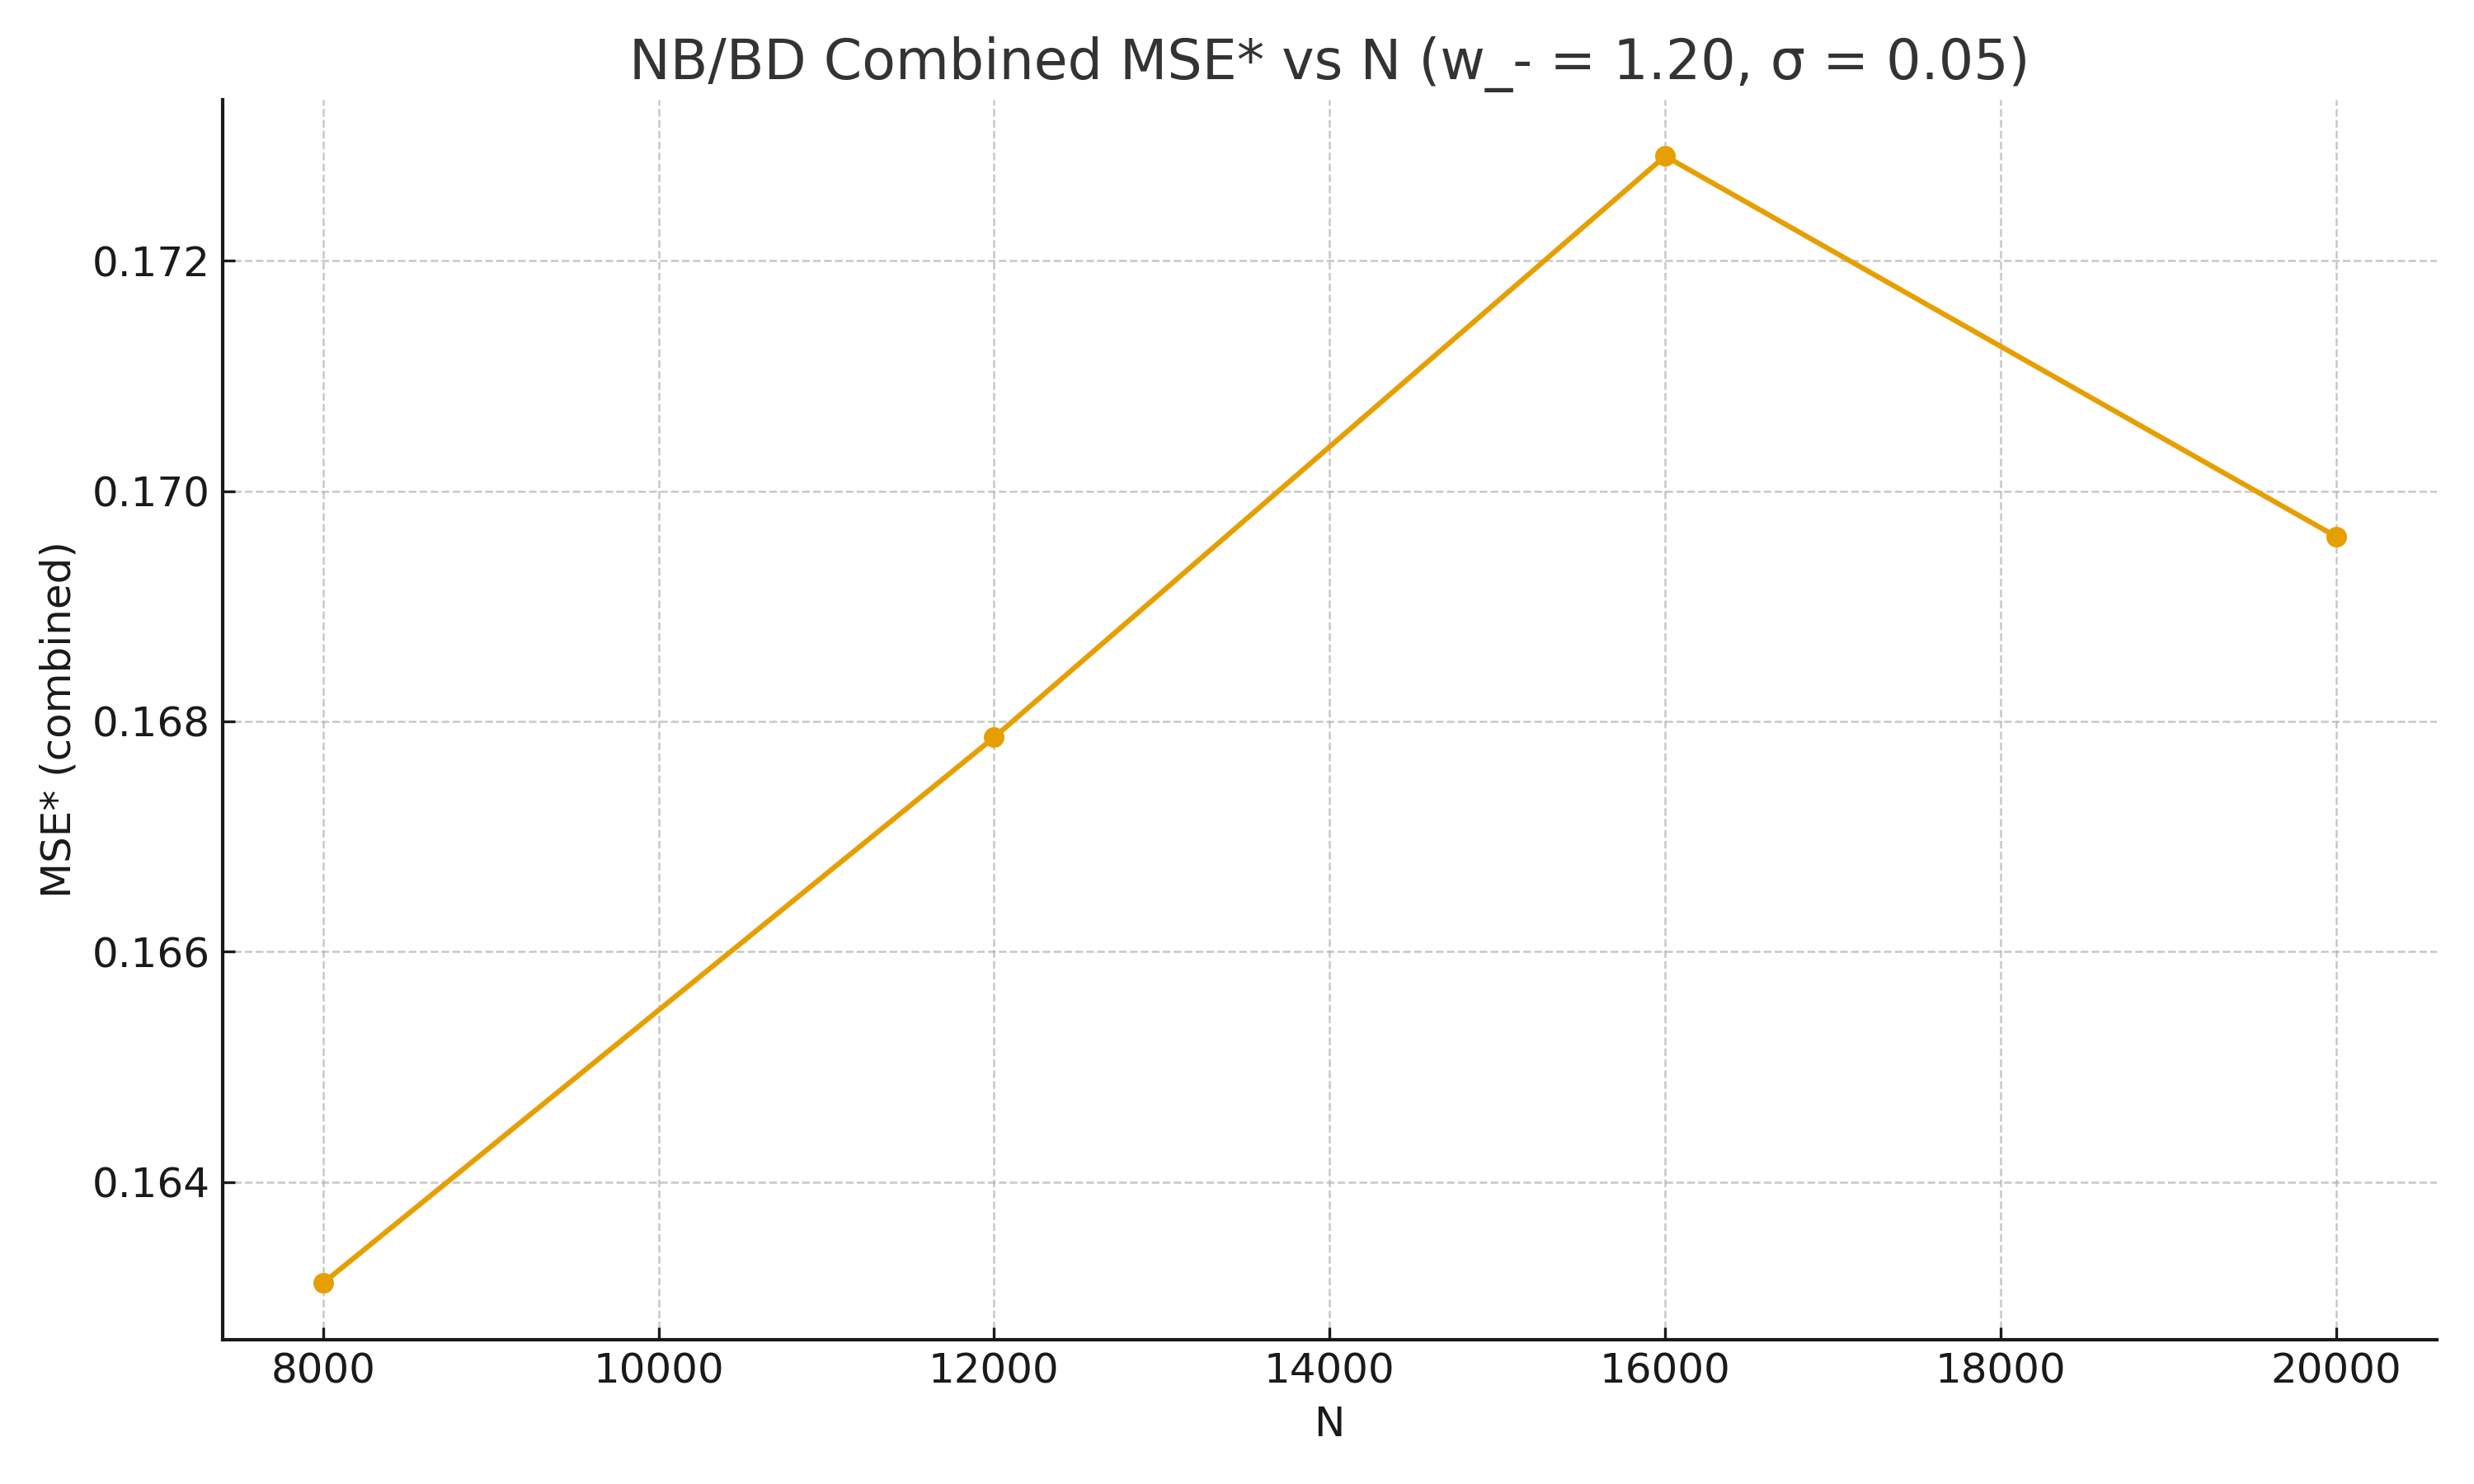
\includegraphics[width=0.75\linewidth]{figures/figure1_mse_star.png}
\caption{Combined $\mathrm{MSE}_\ast$ vs $N$ under $w_-=1.20$, $\sigma=0.05$.}
\end{figure}

\begin{figure}[h]
\centering
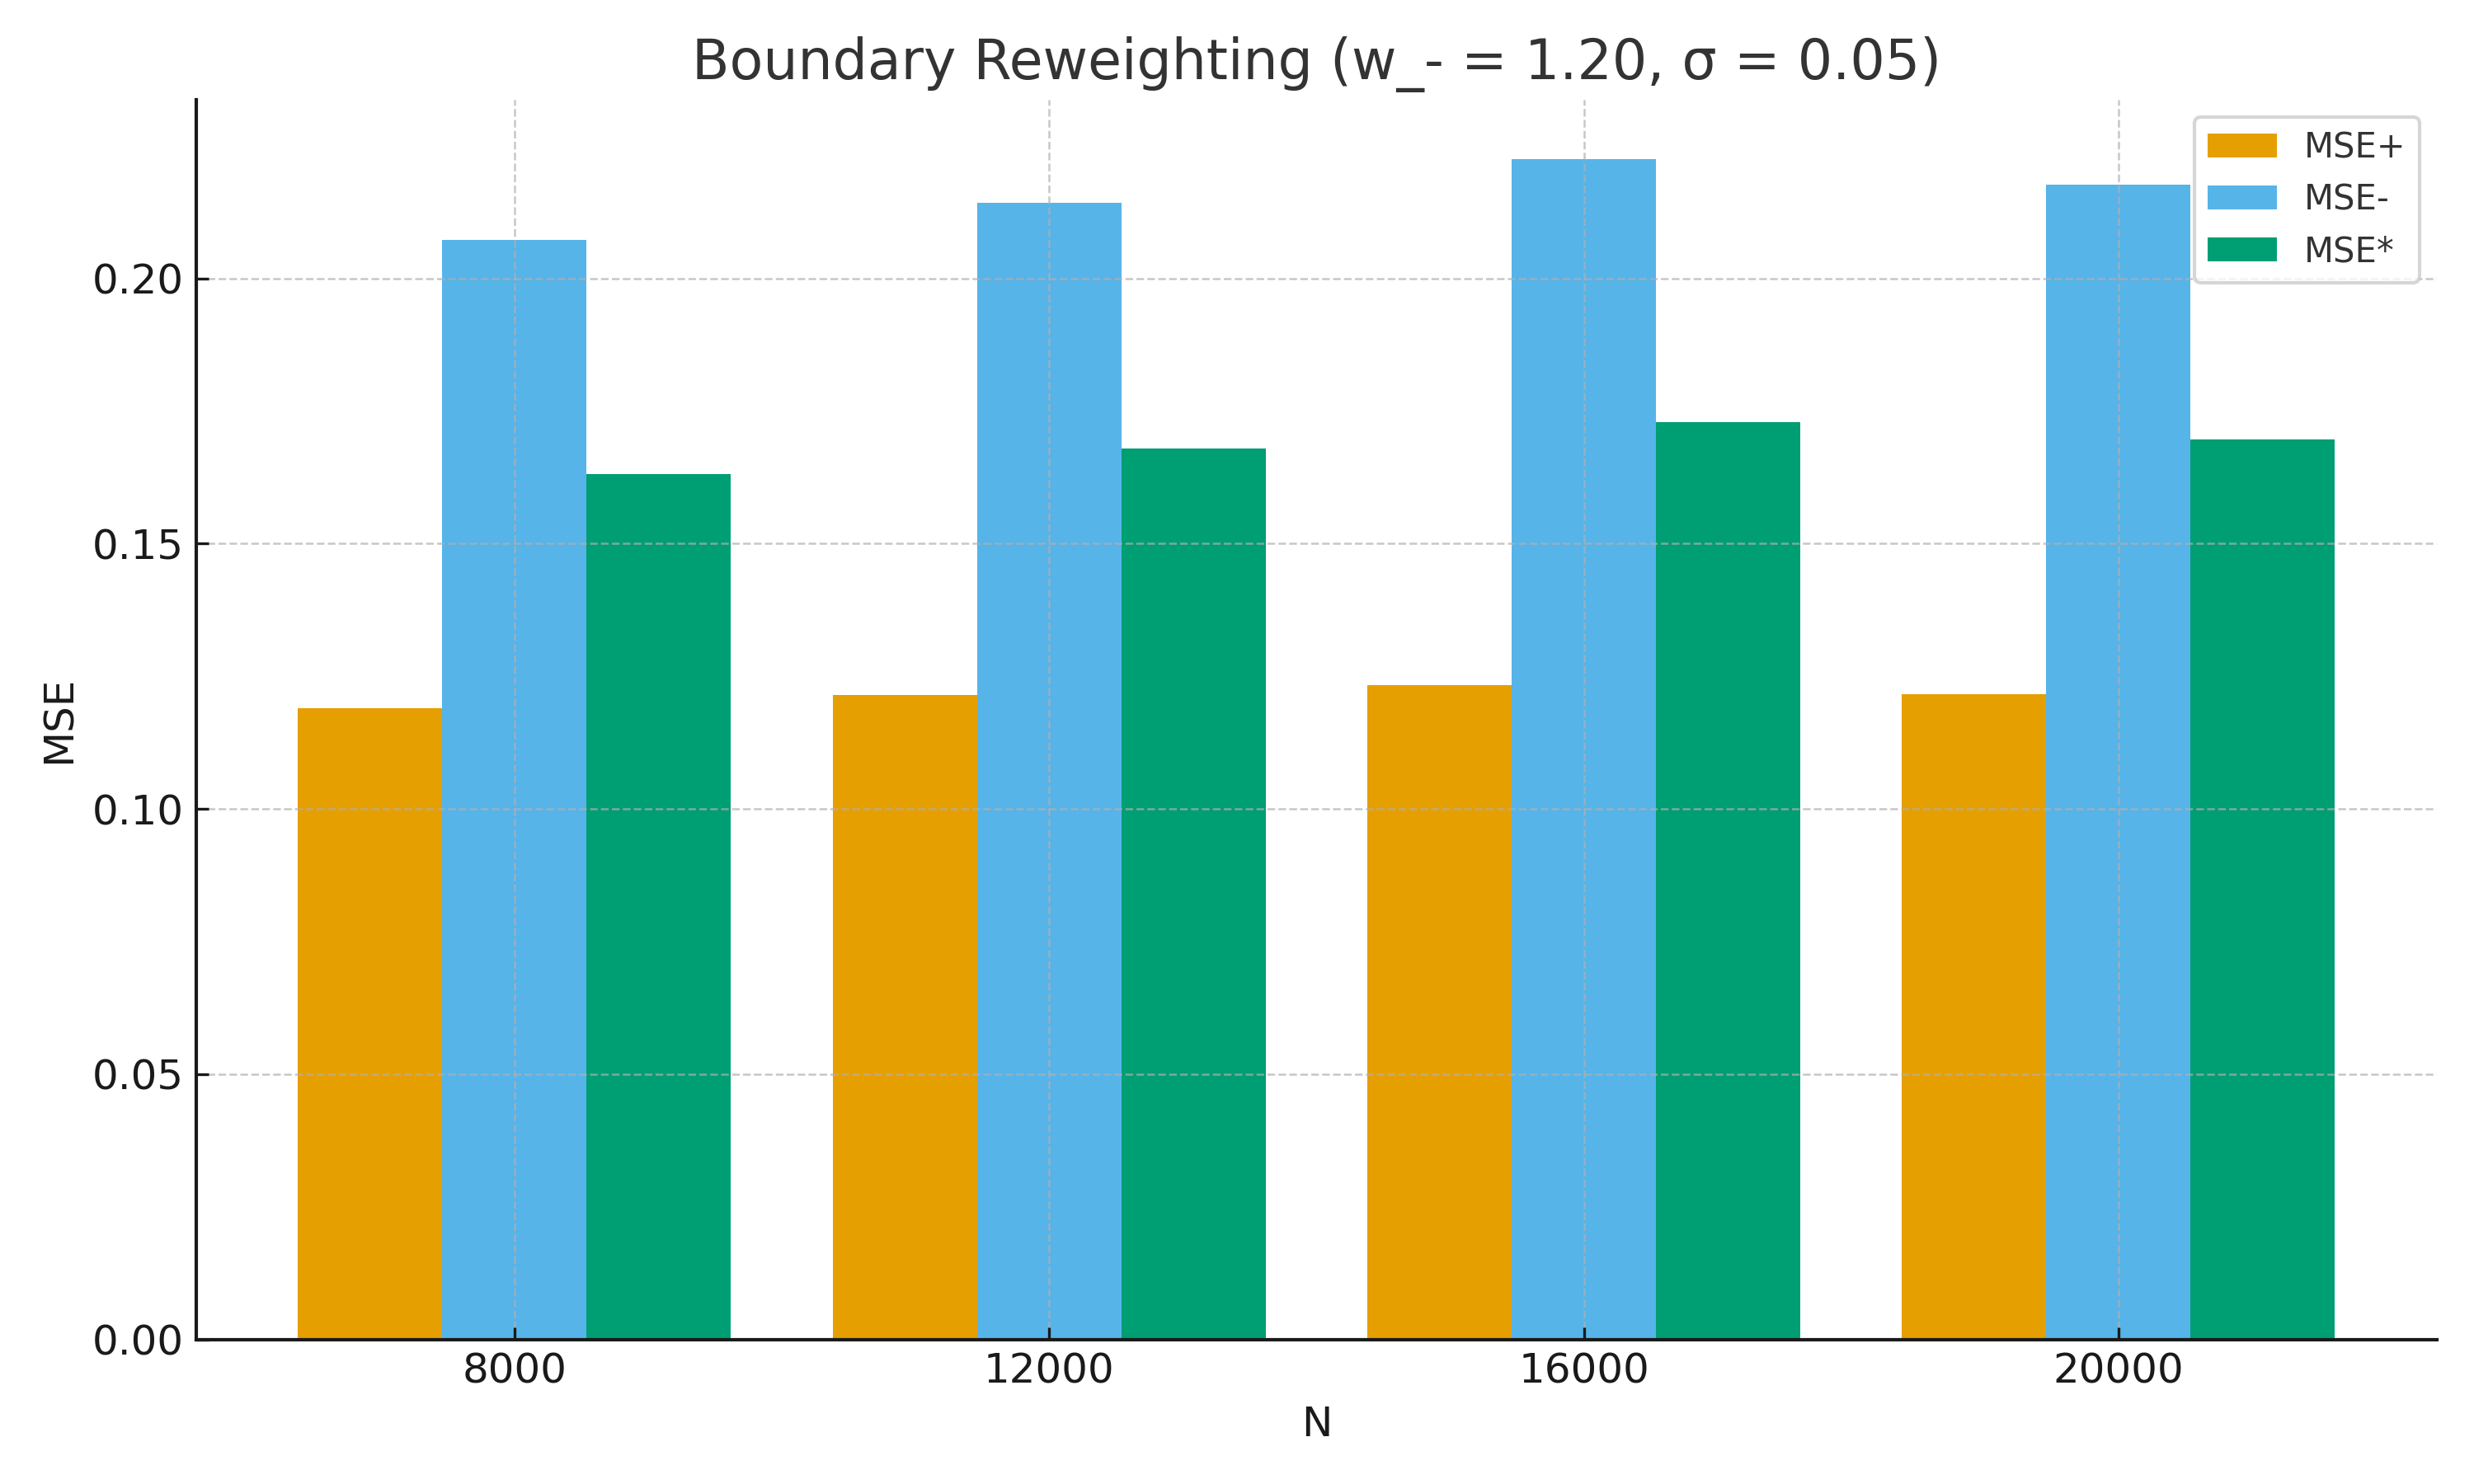
\includegraphics[width=0.75\linewidth]{figures/figure2_boundaries.png}
\caption{Boundary comparison: $\mathrm{MSE}_+$, $\mathrm{MSE}_-$ and $\mathrm{MSE}_\ast$.}
\end{figure}

\section{Scope and Remarks}
The decay \eqref{eq:hilbert} ensures stability of the NB/BD normal equations, but does not prove RH.
Our figures are rebuilt from recorded values and serve as a visual cross-check of the consolidated framework.
Further progress requires larger $N$ and sharper explicit constants.

\end{document}
